% =============================================================================
% COPYRIGHT AND DISCLAIMER
% =============================================================================
% This file is provided as a convenience template for competition participants.
% By using it, you accept full responsibility for compliance with all applicable
% copyright, licensing, and usage rules of the Association for Computing
% Machinery (ACM) and of any LaTeX packages you load (including, without
% limitation, the "acmart" document class and related ACM materials).
%
% Consult ACM's official publication, template, and copyright policies before
% using this setup for any purpose other than this competition. Do not assume
% that this template may be reused, redistributed, or submitted elsewhere
% without independently verifying ACM's current rules.
%
% Use of the "acmart" class, the "sigconf" option, or ACM-style formatting in
% this template does NOT mean that this report, this competition, its organizers,
% or any resulting PDF is sponsored, endorsed, affiliated with, or published by
% ACM. ACM trademarks and branding remain the property of ACM.
%
% Template packages live in preamble.tex.
% Citations live in main.bib. Edit this file with your paper content.
% =============================================================================

\documentclass[sigconf]{acmart}
\input{preamble}
\usepackage{tikz}
\usetikzlibrary{positioning,arrows.meta}

% Guide styling: \guideStyletrue = show gray italic hints; \guideStylefalse = omit them
% \guideStyletrue
\guideStylefalse

\begin{document}

\title{Full-Resolution U-Net with Morphological Instance Grouping for Solar Filament Segmentation}
\subtitle{A Solution to the Solar Filament Segmentation Challenge 2026} % DO NOT CHANGE


\author{Kushagra Tomar}
\affiliation{%
  \institution{Independent Researcher}
  \city{TODO-City}
  \country{TODO-Country}
}
\email{kushagratomar2016@gmail.com}

\begin{abstract}
    This report describes our solution to the Solar Filament Segmentation Challenge~2026, a Kaggle competition on automatic segmentation of solar filaments in GONG H-$\alpha$ observations. Our pipeline has two stages. First, a U-Net with an ImageNet-pretrained EfficientNet-B3 encoder predicts a per-pixel filament probability on the full $2048\times2048$ image, averaged over four flipped views. Second, a short morphological post-processing chain turns this probability map into filament instances: thresholding, closing and hole filling, grouping nearby fragments through the connected components of a dilated mask, and discarding small or low-confidence components. A single model trained for 1.6~hours on one NVIDIA T4 GPU reaches a Panoptic Quality (PQ) of 0.36 on the public leaderboard and processes a test image in 1.2~seconds. The code, trained weights and a notebook that regenerates the submission without retraining are publicly available.
\end{abstract}

\maketitle

\ifguideStyle
\noindent{\color{gray!65}\itshape
Guide mode is on.}
\par\medskip
\fi


% ==================================== %
%              INTRODUCTION            %
% ==================================== %
\section{Introduction}
    This report goes over the details of our submitted solution to the Solar Filament Segmentation Challenge~2026 \cite{filament-segmentation-2026}. The challenge, launched on July~10,~2026, is organized by the Earth-Space AI Research (ESAIR) Lab\footnote{\href{https://www.esairlab.com/home}{www.esairlab.com/}}. This challenge utilizes the MAGFiLO dataset for evaluation of the segmentation algorithms \cite{ahmadzadeh2024dataset}. Submissions are ranked by Panoptic Quality (PQ) \cite{kirillov2019panoptic}, which rewards accurate masks but also penalizes every unmatched prediction and ground-truth filament. Fragmenting one filament into several pieces, or merging several filaments into one, therefore costs as much as a missed detection.

    We chose a deliberately simple design: a single semantic segmentation network followed by deterministic post-processing. The network is responsible for \emph{where} filament material is, at full image resolution so that thin structures are kept. The post-processing is responsible for \emph{which} pixels belong to the same filament. Every step of the pipeline is contained in one Jupyter notebook\footnote{\url{https://github.com/KushagraTomar/Solar-Filament-Segmentation-Challenge-2026}}, which loads the released weights and regenerates the submission file without retraining.


% ==================================== %
%              METHODOLOGY             %
% ==================================== %
\section{Methodology}\label{sec:methodology}
    Figure~\ref{fig:pipeline} summarizes the end-to-end pipeline. All hyperparameters are listed in Table~\ref{tab:hyper}.

\begin{figure*}[t]
  \centering
  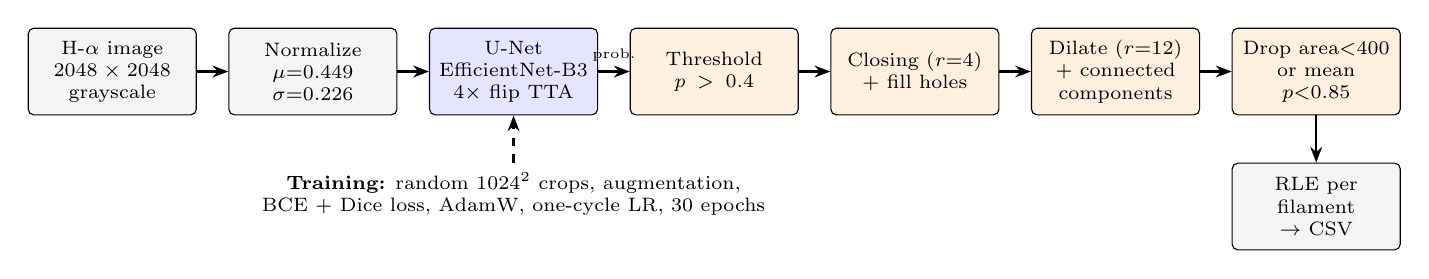
\begin{tikzpicture}[
      node distance=4mm,
      box/.style={draw, rounded corners=2pt, align=center, font=\scriptsize,
                  minimum height=11mm, text width=19mm, fill=gray!8},
      model/.style={box, fill=blue!10},
      post/.style={box, fill=orange!12},
      arr/.style={-{Stealth[length=2mm]}, thick}]
    \node[box]   (in)   {H-$\alpha$ image\\$2048\times2048$\\grayscale};
    \node[box,   right=of in]   (norm) {Normalize\\$\mu{=}0.449$\\$\sigma{=}0.226$};
    \node[model, right=of norm] (net)  {U-Net\\EfficientNet-B3\\4$\times$ flip TTA};
    \node[post,  right=of net]  (thr)  {Threshold\\$p > 0.4$};
    \node[post,  right=of thr]  (cls)  {Closing ($r{=}4$)\\+ fill holes};
    \node[post,  right=of cls]  (cc)   {Dilate ($r{=}12$)\\+ connected\\components};
    \node[post,  right=of cc]   (flt)  {Drop area${<}400$\\or mean $p{<}0.85$};
    \node[box,   below=6mm of flt] (out) {RLE per filament\\$\rightarrow$ CSV};
    \draw[arr] (in) -- (norm);
    \draw[arr] (norm) -- (net);
    \draw[arr] (net) -- node[above, font=\tiny] {prob.} (thr);
    \draw[arr] (thr) -- (cls);
    \draw[arr] (cls) -- (cc);
    \draw[arr] (cc) -- (flt);
    \draw[arr] (flt) -- (out);
    \node[font=\scriptsize, below=6mm of net, align=center] (train)
      {\textbf{Training:} random $1024^2$ crops, augmentation,\\BCE + Dice loss, AdamW, one-cycle LR, 30 epochs};
    \draw[arr, dashed] (train) -- (net);
  \end{tikzpicture}
  \caption{End-to-end pipeline. Blue: learned model. Orange: deterministic post-processing that converts the probability map into filament instances. All radii and areas are in pixels of the original $2048\times2048$ image.}
  \label{fig:pipeline}
\end{figure*}

\subsection{Data and Sampling}
    The training set contains 707 H-$\alpha$ images with 1154 annotator batches; an image may have been labelled independently by up to three annotators. We use each annotator batch as a separate training sample and merge all filament polygons of a batch into one binary mask. Images annotated by several experts are therefore seen several times per epoch with slightly different labels, which acts as a mild form of label smoothing at filament boundaries. Only the provided H-$\alpha$ images and segmentation polygons are used; no external data and no other annotation fields (bounding boxes, spines, labels) are used.

    The final model is trained on all 1154 samples with no held-out split, so that every annotated image contributes to the released weights. The post-processing parameters (Section~\ref{sec:post}) were selected by a grid search on validation PQ using a held-out split in earlier development experiments, and were then kept fixed.

\subsection{Pre-processing}
    Images are read as 8-bit grayscale and normalized with the grayscale ImageNet statistics ($\mu=0.449$, $\sigma=0.226$). We do not resize, crop the solar disk, or correct limb darkening: the network sees the original pixels, which keeps narrow filaments and barbs that would be lost by downsampling a $2048\times2048$ image.

\subsection{Segmentation Model}
    We use a U-Net \cite{ronneberger2015unet} with an EfficientNet-B3 encoder \cite{tan2019efficientnet} pretrained on ImageNet, as implemented in \texttt{segmentation\_models\_pytorch} \cite{iakubovskii2019smp}. The first convolution is adapted to a single input channel, and the decoder ends in a single output channel holding the filament logit. The model has about 13~M parameters (53~MB in 32-bit floats). Because it is fully convolutional, it is trained on crops but applied to the whole image at inference.

\subsection{Training}
    Each sample is augmented with a random $1024\times1024$ crop, horizontal and vertical flips, $90^\circ$ rotations, a mild affine transform (scale $0.9$--$1.1$, rotation $\pm15^\circ$), brightness/contrast and gamma jitter, and occasional Gaussian blur, using Albumentations \cite{buslaev2020albumentations}. The loss is the sum of binary cross-entropy and soft Dice loss \cite{milletari2016vnet}; the Dice term counteracts the strong foreground--background imbalance, since filaments cover a small fraction of the disk. We optimize with AdamW \cite{loshchilov2019adamw} and a one-cycle learning-rate schedule \cite{smith2019superconvergence} in mixed precision for 30 epochs (288 iterations of batch size 4 per epoch). We keep the weights from the final epoch, where the schedule ends at a near-zero learning rate. The training loss falls from 1.85 in the first epoch to 0.31 in the last. Training takes 1~h~37~min on a single NVIDIA T4 (16~GB).

\begin{table}[t]
  \caption{Hyperparameters of the final pipeline.}
  \label{tab:hyper}
  \small
  \begin{tabular}{ll}
    \toprule
    Setting & Value \\
    \midrule
    Encoder / weights & EfficientNet-B3 / ImageNet \\
    Input & 1 channel, full resolution \\
    Training crop / batch size & $1024^2$ / 4 \\
    Optimizer / LR / weight decay & AdamW / $3\times10^{-4}$ / $10^{-4}$ \\
    Schedule / epochs & one-cycle / 30 \\
    Loss & BCE + Dice \\
    Test-time augmentation & 4 flips (none, H, V, H+V) \\
    Threshold $\tau$ & 0.4 \\
    Closing radius $r_c$ & 4 px \\
    Merge (dilation) radius $r_m$ & 12 px \\
    Minimum area $A_{\min}$ & 400 px \\
    Minimum mean probability $c_{\min}$ & 0.85 \\
    Random seed & 42 \\
    \bottomrule
  \end{tabular}
\end{table}

\subsection{Inference}
    The whole $2048\times2048$ image is passed through the network four times (original, horizontal flip, vertical flip, both), each output is flipped back, and the four sigmoid probability maps are averaged into a single map $P$.

\subsection{Post-processing: from Pixels to Filaments}\label{sec:post}
    PQ is computed on instances, so the probability map must be split into individual filaments. With $D_r$ a disk of radius $r$, we compute:
    \begin{enumerate}
      \item \textbf{Threshold}: $M = [P > \tau]$.
      \item \textbf{Smooth}: $M \leftarrow \mathrm{fill}(M \bullet D_{r_c})$, a morphological closing followed by hole filling. The MAGFiLO masks are rasterized polygons with no holes, so small gaps and holes in $M$ can only be errors.
      \item \textbf{Group}: label the 8-connected components of the dilated mask $M \oplus D_{r_m}$, then keep the labels only on the pixels of $M$. Fragments separated by less than about $2r_m$ pixels share one identifier, which reduces one-to-many matches, while each instance keeps its undilated shape. An instance may therefore consist of several disconnected parts.
      \item \textbf{Filter}: discard an instance if its area is below $A_{\min}$ or its mean probability is below $c_{\min}$. In PQ, every false-positive instance increases the denominator, so we prefer to drop small or uncertain blobs.
    \end{enumerate}
    Each remaining instance is encoded as COCO run-length counts with \texttt{pycocotools} \cite{lin2014coco} and written as one row of the submission file. The few test images with no detection receive a single empty mask, so that every image appears in the file. Figure~\ref{fig:example} shows the result on a test image.

\begin{figure}[t]
  \centering
  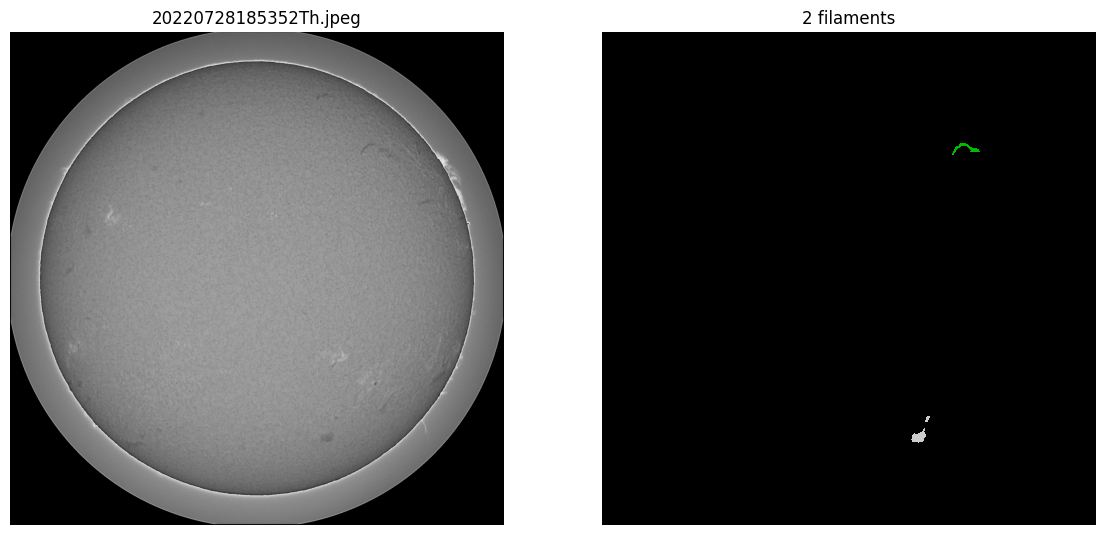
\includegraphics[width=\columnwidth]{figures/sample_prediction.png}
  \caption{Test image 20220728185352Th (left) and the predicted instances (right; one color per filament). The lower instance shows the grouping step: two nearby fragments are assigned the same identifier.}
  \label{fig:example}
\end{figure}


% ==================================== %
%              EVALUATION              %
% ==================================== %
\section{Evaluation}\label{sec:evaluation}
\subsection{Strategy}
    The final model was evaluated on the hidden test set through the competition leaderboard, which reports PQ on about half of the 180 test images. Test ground truth is not available to participants, and the released model uses all annotated images for training. We therefore report the leaderboard score, the computational cost, a reproducibility check, and descriptive statistics of the predictions (Tables~\ref{tab:results} and~\ref{tab:preds}). We do not report per-image Dice or IoU distributions or error bars on PQ, because they would require ground truth that the final model has not seen.

\begin{table}[t]
  \caption{Results of the submitted pipeline (single NVIDIA T4 GPU).}
  \label{tab:results}
  \small
  \begin{tabular}{ll}
    \toprule
    Metric & Value \\
    \midrule
    Public leaderboard PQ & 0.36 \\
    Training time & 1 h 37 min \\
    Inference, 180 test images & 222 s (1.23 s / image) \\
    Model size & $\approx$13 M parameters, 53 MB \\
    \bottomrule
  \end{tabular}
\end{table}

\begin{table}[t]
  \caption{Statistics of the predictions on the 180 test images.}
  \label{tab:preds}
  \small
  \begin{tabular}{ll}
    \toprule
    Quantity & Value \\
    \midrule
    Predicted filaments & 1037 \\
    Filaments per image, mean $\pm$ SD & $5.76 \pm 3.36$ \\
    Filaments per image, median (IQR) & 6 (3--8), max 14 \\
    Images with no detection & 4 \\
    Filament area, median (IQR) & 1542 (851--2792) px \\
    Filament area, range & 400--20788 px \\
    \bottomrule
  \end{tabular}
\end{table}

\subsection{Computational Efficiency}
    The inference time in Table~\ref{tab:results} covers the whole per-image pipeline: reading the image, four forward passes, post-processing and RLE encoding. A single network with no ensembling, a fixed-cost post-processing chain and no resizing keep the method simple and fast.

\subsection{Reproducibility}
    The submitted file was generated by the released notebook from the released weights, without retraining. We compared it with the predictions written at the end of the training run, made with the same weights in memory. Both contain the same 1041 rows. Of these masks, 968 are bit-identical; the remaining 73 differ only by a few boundary pixels (104 of 2.38~M predicted pixels, IoU $\geq 0.994$ for every mask). We attribute these differences to non-deterministic mixed-precision GPU arithmetic; they do not change the number of filaments.

\subsection{Strengths and Weaknesses}
    \textbf{Strengths.} (i)~Full-resolution training and inference keep thin filaments that downsampling would erase. (ii)~The pipeline is small and fast: one network, flip TTA and five post-processing steps with interpretable parameters. (iii)~Training on every annotator batch uses all expert labels without having to resolve disagreements between them. (iv)~Results are reproducible from the released weights.

    \textbf{Weaknesses.} (i)~The network is trained for semantic segmentation only; filament identity is decided by a fixed merge radius. This can join two distinct filaments that lie close together (many-to-one), or fail to join a filament with gaps larger than $2r_m$ (one-to-many). (ii)~The minimum area of 400~px removes small filaments together with noise. (iii)~One global threshold is used for images from six GONG sites with different seeing conditions and contrast. (iv)~Without an internal validation of the final model, we cannot attach uncertainty to the leaderboard score.

    \textbf{Possible improvements.} K-fold cross-validation would provide per-image PQ, Dice and IoU distributions with bootstrap confidence intervals, and a fold ensemble would likely improve accuracy. Predicting instance cues directly, for example filament spines or boundaries, would let grouping depend on filament orientation and continuity instead of distance alone. Per-site normalization or threshold calibration could reduce the effect of varying image quality.


% ==================================== %
%            ACKNOWLEDGMENT            %
% ==================================== %
\section{Acknowledgment}\label{sec:acknowledgment}
    % Do not change
    The organization of the Filament Segmentation Challenge 2026 is partially supported by the U.S. National Science Foundation (NSF) under Grant No. 2209912 and 2433781, directorate for Computer and Information Science and Engineering (CSE), and Office of Advanced Cyberinfrastructure (OAC), and Grant No. 2511630, AST Division Of Astronomical Sciences and MPS Directorate for Mathematical and Physical Sciences.

    The Filament Segmentation Challenge 2026 is sponsored by the U.S. National Science Foundation (NSF) National Solar Observatory (NSO).

    This work utilizes GONG data obtained by the NSO Integrated Synoptic Program, managed by the National Solar Observatory, which is operated by the Association of Universities for Research in Astronomy (AURA), Inc. under a cooperative agreement with the National Science Foundation and with contribution from the National Oceanic and Atmospheric Administration. The GONG network of instruments is hosted by the Big Bear Solar Observatory, High Altitude Observatory, Learmonth Solar Observatory, Udaipur Solar Observatory, Instituto de Astrofísica de Canarias, and Cerro Tololo Interamerican Observatory.

\bibliographystyle{ACM-Reference-Format}
\bibliography{main}

\end{document}
